%%%%%%%%%%%%%%%%%%%%%%%%%%%%%%%%%%%%%%%%%
% Daily Laboratory Book
% LaTeX Template
% Version 1.0 (4/4/12)
%
% This template has been downloaded from:
% http://www.LaTeXTemplates.com
%
% Original author:
% Frank Kuster (http://www.ctan.org/tex-archive/macros/latex/contrib/labbook/)
%
% Important note:
% This template requires the labbook.cls file to be in the same directory as the
% .tex file. The labbook.cls file provides the necessary structure to create the
% lab book.
%
% The \lipsum[#] commands throughout this template generate dummy text
% to fill the template out. These commands should all be removed when 
% writing lab book content.
%
% HOW TO USE THIS TEMPLATE 
% Each day in the lab consists of three main things:
%
% 1. LABDAY: The first thing to put is the \labday{} command with a date in 
% curly brackets, this will make a new page and put the date in big letters 
% at the top.
%
% 2. EXPERIMENT: Next you need to specify what experiment(s) you are 
% working on with an \experiment{} command with the experiment shorthand 
% in the curly brackets. The experiment shorthand is defined in the 
% 'DEFINITION OF EXPERIMENTS' section below, this means you can 
% say \experiment{pcr} and the actual text written to the PDF will be what 
% you set the 'pcr' experiment to be. If the experiment is a one off, you can 
% just write it in the bracket without creating a shorthand. Note: if you don't 
% want to have an experiment, just leave this out and it won't be printed.
%
% 3. CONTENT: Following the experiment is the content, i.e. what progress 
% you made on the experiment that day.
%
%%%%%%%%%%%%%%%%%%%%%%%%%%%%%%%%%%%%%%%%%

%----------------------------------------------------------------------------------------
%	PACKAGES AND OTHER DOCUMENT CONFIGURATIONS
%----------------------------------------------------------------------------------------

\documentclass[idxtotoc,hyperref,openany,oneside]{files/reverse} % 'openany' here removes the gap page between days, erase it to restore this gap; 'oneside' can also be added to remove the shift that odd pages have to the right for easier reading

\usepackage[ 
  backref=page,
  pdfpagelabels=true,
  plainpages=false,
  colorlinks=true,
  bookmarks=true,
  pdfview=FitB]{hyperref} % Required for the hyperlinks within the PDF
  
\usepackage{booktabs} % Required for the top and bottom rules in the table
\usepackage{float} % Required for specifying the exact location of a figure or table
\usepackage{graphicx} % Required for including images2
\usepackage{listings} % Used for programs' listings
\usepackage{tcolorbox} % For textboxes

\usepackage[english,russian]{babel}
\usepackage[utf8]{inputenc}
\usepackage[T2A]{fontenc}

\newcommand{\HRule}{\rule{\linewidth}{0.5mm}} % Command to make the lines in the title page
\setlength\parindent{0pt} % Removes all indentation from paragraphs

%----------------------------------------------------------------------------------------
%	DEFINITION OF EXPERIMENTS
%----------------------------------------------------------------------------------------

\newexperiment{easy1}{Check the license!}
\newexperiment{easy2}{Guess the password}
\newexperiment{medium}{Cryptowallet}
\newexperiment{hard}{Friendly VM}
\newexperiment{reallife}{Let's GO for cookies}

%---------------------------------------------------------------------------------------

\begin{document}

%----------------------------------------------------------------------------------------
%	TITLE PAGE
%----------------------------------------------------------------------------------------

\frontmatter % Use Roman numerals for page numbers
\title{
\begin{center}
\HRule \\[0.4cm]
{\Huge \bfseries CTF Code \\[0.5cm] \Large Writeups}\\[0.4cm] % Degree
\HRule \\[1.5cm]
\end{center}
}
\author{\Huge Reverse Engineering \\ \\[2cm]} % Your name and email address
\maketitle

\tableofcontents

\mainmatter % Use Arabic numerals for page numbers

%----------------------------------------------------------------------------------------
%	LAB BOOK CONTENTS
%----------------------------------------------------------------------------------------

% Blank template to use for new days:

%\labday{Day, Date Month Year}

%\experiment{}

%Text

%-----------------------------------------

%\experiment{}

%Text

%----------------------------------------------------------------------------------------

\labday{Easy}

\experiment{easy1}

\textbf{Теги:} Java, License key\vspace{\baselineskip}

\begin{tcolorbox}
<условие задачи>
\end{tcolorbox}

Нам дается программа на Java, которая хочет какую-то лицензию. Самое время ее разреверсить и посмотреть, что же там за лицензия нам нужна. Так как это Java, то можно восстановить исходный код с точностью до имен переменных с помощью любого декомпилятора. В райтапе будет использоваться JD-GUI. После открытия файла видим, что он совсем небольшой и состоит всего из трех классов:
\begin{figure}[H]
\begin{center}
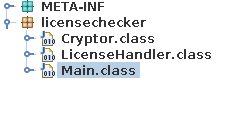
\includegraphics[width=0.7\linewidth]{files/java-classes}
\end{center}
\caption{Java изнутри}
\label{fig:java-classes}
\end{figure}

После рассмотрения \verb|Main|'a понимаем, что это просто драйвер и ничего связанного с лицензией или ее обработкой не делает. С классом \verb|LicenseHandler| ситуация интереснее, но тоже ничего нужного нам - ни расшифровки, ни каких-либо проверок. Просто чтение из класса и обращение к классу \verb|Cryptor|, который, судя по всему, нам и нужен. Декомпилируем и смотрим:
\begin{figure}[H]
\begin{center}
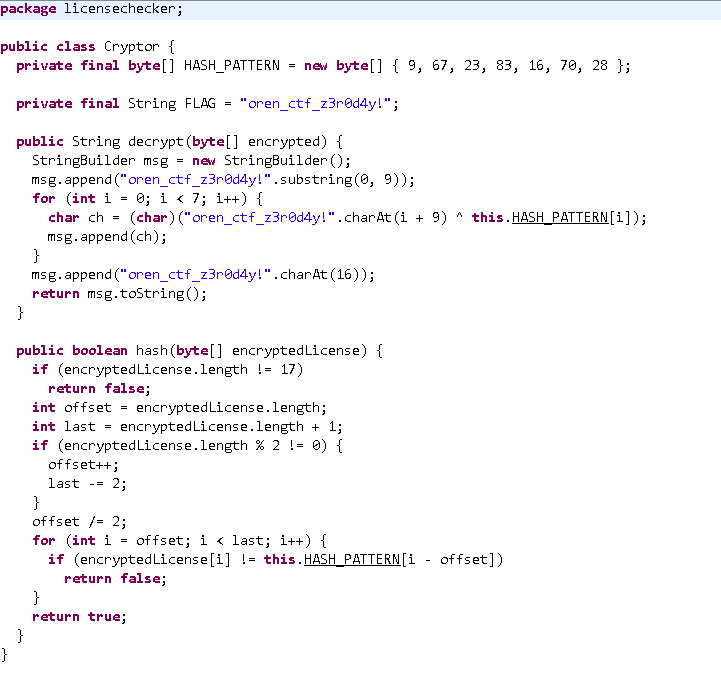
\includegraphics[width=0.7\linewidth]{files/java-cryptor}
\end{center}
\caption{Когда создал свою крипту}
\label{fig:java-classes}
\end{figure}

С первого взгляда флаг лежит прямо перед нами. Но это как-то слишком просто даже для easy-задачи. Посмотрим чуть ниже. Дейсвительно, сначала происходит какая-то проверка хэша. Если посмотреть внимательнее - никаких хешей нет. Сначала проверяем, что длина лицензии 17 символов, потом просто массив байтиков, с 9 по 15 элементы, сверяется с константой \verb|HASH_PATTERN|. После чего в функции \verb|decrypt| собирается флаг - обертка остается без изменений, а вот 7 символов ксорятся с \verb|HASH_PATTERN|. После чего совсем не сложно написать простенький скрипт для ксора или (что еще проще) написать скрипт, который "сгенерирует" лицензию и скормить ее программе:
\begin{lstlisting}[language=Python, caption=Генератор лицензии]
#!/usr/bin/env python3
# -*- coding: utf-8 -*-

def main():
    xored = ['\x00', '\x00', '\x00', '\x00', '\x00', '\x00', '\x00',
    '\x00', '\x00', '\x09', '\x15', '\x17', '\x0c', '\x10', '\x13', 
    '\x1c', '\x00']

    with open('license.bin', 'wb') as licensefile:
        for xb in xored:
            licensefile.write(bytes(xb, 'utf-8'))


if __name__ == "__main__":
    main()
\end{lstlisting}

И получаем флаг:
\begin{figure}[H]
\begin{center}
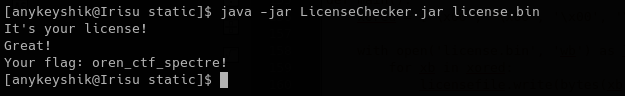
\includegraphics[width=0.7\linewidth]{files/java-flag}
\end{center}
\caption{Привет от Intel'a}
\label{fig:java-flag}
\end{figure}

%-----------------------------------------

\experiment{easy2}

\textbf{Теги:} C, ELF32, strip, dynamic, several ways of solve\vspace{\baselineskip}

\begin{tcolorbox}
<условие задачи>
\end{tcolorbox}

Программа расшифровывает флаг и ждет от нас пароля, чтобы отдать его нам.
\begin{figure}[H]
\begin{center}
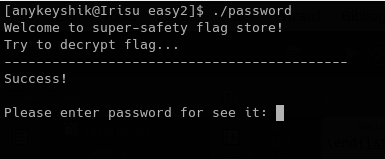
\includegraphics[width=0.5\linewidth]{files/enigma-hello}
\end{center}
\label{fig:enigma-hello}
\end{figure}

Посомтрим, что же в этот момент происходит внутри:
\begin{figure}[H]
\begin{center}
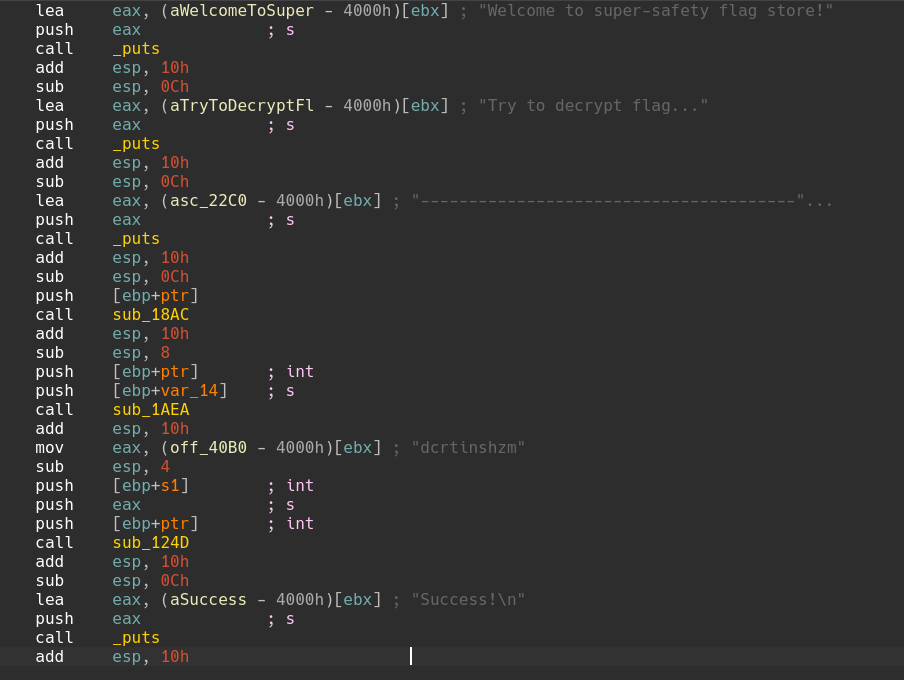
\includegraphics[width=1.0\linewidth]{files/enigma-asm}
\end{center}
\label{fig:enigma-asm}
\end{figure}

Глядя на этот листинг становится понятно, что действительно вызываются две функции. Судя по всему, одна из них для инициализации ключа, вторая для расшифровки. Таким образом, наш флга лежит в памяти еще до того, как программа спросила пароль. И тут появляется огромное количество возможных решений: к примеру, сдампить процесс, в дебаггере посмотреть содержимое кучи или, самый простой, - воспользоваться утилитой \verb|ltrace|, чтобы отследить все библиотечные вызовы - они тут есть, в этом можно убедиться, если посмотреть, что импортирует программа. Есть второй, более сложный путь решения, - увидеть, что пароль сравнивается с помощью функции \verb|strcmp| и поменять переход \verb|jnz| на \verb|jz| и, таким образом, при вводе неправильного пароля переходить на ветку, где программма печатает флаг. Ниже приведено решение с использованием \verb|ltrace|:
\begin{figure}[H]
\begin{center}
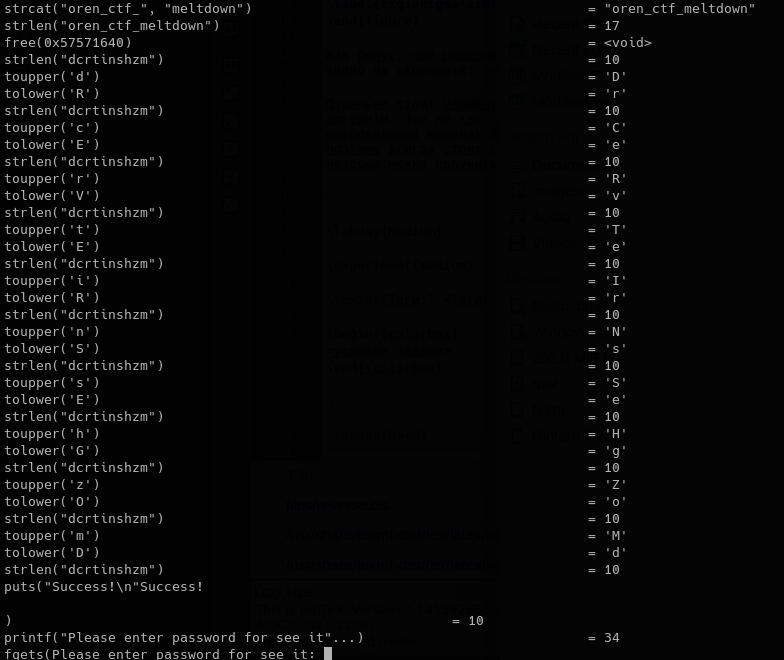
\includegraphics[width=1.0\linewidth]{files/enigma-ltrace}
\end{center}
\label{fig:enigma-asm}
\end{figure}

Как бонус, при решении через \verb|ltrace| можно также получить и пароль - это хорошо видно на скриншоте: \verb|reversegod|.

Отдельно стоит упомянуть решение "в лоб"{} - просто посидеть и прореверсить весь алгоритм. Это не так сложно - в данном случае был использован алгоритм, применявшийся в шифровальных машинах Энигма. Но для простой задачи это очень времязатратная операция, поэтому всегда стоит ставить в соответствие временные затраты и количество баллов, которые можно получить за задачу.

%----------------------------------------------------------------------------------------

\labday{Medium}

\experiment{medium}

\textbf{Теги:} C++, ELF64, strip, dynamic\vspace{\baselineskip}

\begin{tcolorbox}
<условие задачи>
\end{tcolorbox}

Суть задания - разбор очень простого бинарного формата файла. Анализируем исполняемый файл и понимает, что он парсит файл кошелька довольно простым образом:
\begin{itemize}
\item Первым байтом файла является размер зашифрованного логина, который лежит после этого байта.
\item Данный байт является инициализирующим значение для генератора гаммы с которой XOR'ится логин.
\item Такой же алгоритм используется для пароля.
\item Достаточно вытащить пароль и логин из кошелька и открыть его с помощью предоставленного исполняемого файла.
\item Теперь мы можем просматривать все поля кошелька, однако нам нужно загрузить свой кошелёк с определённым балансом.
\item Разбираем формат кошелька дальше, это не сложно делать, т.к. внутри бинарника есть функция вывода информации о кошельке, что позволяет достаточно просто и быстро определить смещения на поля и увидеть как они обрабатываются.
\item Баланс сохраняется в 4 байта после пароля и "шифруется" путём XOR'а с константой 0xdeadbeef
\item После загрузки кошелька с верным балансом, скорее всего, будет получено уведомление о том, что количество последних операций должно быть выше 16.
\item Операции сохраняются ещё проще. После баланса идёт количество операций, а следующий байт это размер операции, все операции сохраняются таким образом и шифруются XOR'ом с размером.
\item После создания операций в необходимом количестве будет получена ошибка, указывающая, что данный кошелёк не приватный. За это отвечает поле "Info".
\item Поле Info ксорится с ключом, который формируется из логина и пароля
\item Помещаем в поле Info строку "Private" (на это явно указано в сообщении об ошибке от сервера)
\item Загружаем кошелёк и покупаем токен.
\item Токен - это и есть флаг.
\end{itemize}

Таким образом, можно написать простой питоновский скрипт, который автоматизирует всю работу и просто "выдаст флаг на блюдечке с голубой коемочкой":
\begin{lstlisting}[language=Python, caption=Генератор кошелька]
#!/usr/bin/env python2
# -*- coding: utf-8 -*-

import sys
import random
import struct
import re

from pwn import *

BLANCE_KEY = 0xdeadbeef
ALPH = 'qwertyuiopasdfghjklzxcvbnmQWERTYUIOPASDFGHJKLZXCVBNM0123456789'

p32 = lambda val : struct.pack( "!L", val  )
templates = ['debiting from this account %d bitcoins to %s account',
             'crediting from %s to a wallet %d bitcoins']


def idg(size = 16, chars = ALPH):
	return ''.join(random.choice(chars) for _ in range(size))


def GenRandomValue(seed):
    return (seed >> 1) & 0xff


def GenGamma(seed, sz):
    gamma = []

    for i in range(0, sz):
        value = GenRandomValue(seed)
        seed += value
        gamma.append(value)

    return gamma


def XorStringWithRandomGamma(string):
	res = ''

	seed = len(string)
	gamma = GenGamma(seed, seed)

	for i in range(len(gamma )):
		res += chr(ord(string[i]) ^ gamma[i])

	return res


class Wallet:
	login = None
	password = None
	balance = None
	last_operations = []
	info = None

	def __init__( self, Username, Password, Info ):
		self.login = Username
		self.password = Password
		self.balance = 13371337
		self.gen_random_operations()

		self.info = Info

	def gen_random_operations(self):
		global templates
		for i in range(0, 17):

			template_id = random.randint(0, 1)

			if template_id == 0:
				self.last_operations.append(
				templates[template_id] 
				% (random.randint(100, 512), idg()))
			else:
				self.last_operations.append(
				templates[template_id] 
				% (idg(), random.randint(100, 512)))

	def pack_operations(self):
		for i in range(len(self.last_operations)):
			operation = list(self.last_operations[i])

			for j in range(len(operation)):
				operation[j] = 
				chr(ord(operation[j]) ^ len(operation))

			self.last_operations[i] = ''.join(operation)

	def pack_info( self, key ):
		self.info = list(self.info)

		for i in range( len(self.info )):
			self.info[i] = 
			chr(ord(self.info[i]) ^ ord(key[i % len(key)]))

		self.info = ''.join(self.info)

	def pack_wallet( self ):
		self.pack_operations()

		res = ''
		# Pack login and password
		res += chr(len(self.login))
		res += XorStringWithRandomGamma(self.login)
		res += chr(len(self.password))
		res += XorStringWithRandomGamma(self.password)

		# Write balance
		res += p32(self.balance ^ BLANCE_KEY)

		# Pack all operations
		if len(self.last_operations) > 0:
			res += chr(len(self.last_operations ))

			for operation in self.last_operations:
				res += chr(len( operation ))
				res += operation
		else:
			res += "\x00\x00\x00\x00"

		self.pack_info(self.login + self.password)

		# Pack info
		if len(self.info) > 0:
			res += chr(len(self.info ))

			res += self.info
		else:
			res += "\x00\x00\x00\x00"

		return res.encode('hex')


if __name__ == "__main__":
    if len(sys.argv) > 2:
		host = sys.argv[1]
		port = int(sys.argv[2])
    else:
		print "Usage: " + sys.argv[0] + " <host> <port>"
		sys.exit(-1)

    login = 'AAAABBBBCCCCDDDD'
    password = login * 2

    wallet = Wallet(login, password, 'Private')
    enc_wallet = wallet.pack_wallet()

    r = remote(host, port)

    log.info("Upload wallet")
    r.sendline("2")

    log.info("Send wallet data")
    r.sendline(enc_wallet)

    log.info("Send login")
    r.sendline(login)

    log.info("Send password")
    r.sendline(password)

    log.info("Set as default")
    r.sendline("Y")

    log.info("Buy token")
    r.sendline("3")

    r.interactive()
\end{lstlisting}

В конце концов получаем флаг \verb|oren_ctf_REvil!|

%----------------------------------------------------------------------------------------

\labday{Hard}

\experiment{hard}

\textbf{Теги:} Python, VM, Several ways of solve\vspace{\baselineskip}

\begin{tcolorbox}
<условие задачи>
\end{tcolorbox}

Нам дана виртуалка и дамп программы. Нужно понять, что же происходит в программе и как можно достать флаг.

\textbf{Изучение кода виртуальной машины.}
Немного изучив код класса \verb|VirtualMachine|, можно понять, что виртуальная машина исполняет какие-то ассемблерные инструкции, придуманные автором (на самом деле, основная их часть — это набор инструкций из архитектуры \verb|ARM|). Также из конструктора видно, что аргументом передаётся память для виртуальной машины (та самая, которая дана в условии).

Виртуальная машина (далее ВМ) парсит байты из \verb|memory| в функции \verb|exec|, тем самым понимая какую инструкцию исполнять и с какими операндами (аргументами, если угодно). Из этого можно придти к тому выводу, что нет смысла пытаться искать флаг в коде виртуальной машине. Очевидно, что сама задача состоит в том, чтобы разобраться что исполняет ВМ и каким образом можно получить флаг.

\textbf{Что же исполняет ВМ.}
Здесь есть несколько подходов к тому, как понять что исполняет ВМ.
\begin{itemize}
\item Ставить дебаг вывод в функции \verb|exec| или в подобных, обрабатывающих ассемблерные инструкции (класс \verb|Assembly|).
\item Поставить брейкпоинты на методах класса \verb|Assembly| и смотреть пошагово.
\end{itemize}

На этом моменте вы можете самостоятельно разобраться в том, что же исполняет ВМ. Я лишь приведу уже готовый ассемблерный код:
\begin{lstlisting}[]
mov   R0, 10839
puts  R0
mov   R0, 8191
gets  R0         ; enter string from stding
mov   R1, 0
mov   R2, 0

start_len_calc:
load  R3B, R0
cmp   R3B, 0       ; calculate length of entered string
je    end_len_calc
inc   R0
inc   R1
jmp   start_len_calc

end_len_calc:
cmp   R1, 12     ; entered_str.length == 12
je    correct_len

print_fail_message:
mov   R0, 10639  ; print fail message
puts  R0
exit

correct_len:
mov   R0, 8203
mov   R1, 8202

add_reverse_loop:
cmp   R1, 8191   ; add reversed string to the entered one
jl    end_adding_loop
load  R4, R1
store R4B, R0
dec   R1
inc   R0
jmp   add_reverse_loop

end_adding_loop:
mov   R2, 0      ; null byte to the end of the new string
store R2B, R0
mov   R1, R0
mov   R0, 8191
mov   R4, 0

start_str_encoding:
cmp   R0, R1            ; encode string like that:
je    end_str_encoding  ; str[i] = (str[i] + 4) ^ "konata"[i % 6]
load  R6B, R0           ; get str[i]
add   R6, 4             ; str[i] + 4
mov   R8, R4
add   R8, 10739
load  R7B, R8           ; "konata"[i % 6]
xor   R6, R7            ; xor them
store R6B, R0           ; put into [R0]
inc   R0
inc   R4
mod   R4, 6
jmp   start_str_encoding

end_str_encoding:
mov R0,   8212
hash_sha1 R0, 9000

mov R0, 9000
mov R1, 10439

strcmp R0, R1
jne print_fail_message

mov R0, 8209
mov R1, 8800

start_middle_substring:
cmp   R0, 8212
je    end_middle_substring
load  R2B, R0
store R2B, R1
inc   R0
inc   R1
jmp   start_middle_substring

end_middle_substring:
mov   R2, 0
store R2, R1

mov R0, 8800
hash_md5 R0, 8900

mov R0, 8900
mov R1, 10339

strcmp R0, R1
jne print_fail_message

mov R0, 8800
mov R1, 8191

start_prefix_substring:
cmp R1, 8209
je end_prefix_substring
load R2B, R1
store R2B, R0
inc R1
inc R0
jmp start_prefix_substring

end_prefix_substring:
mov R0, 0
store R0B, R1

mov R0, 8800

start_encode_prefix:
cmp R0, 8818
je end_encode_prefix
load R1B, R0
xor R1, 42
store R1B, R0
inc R0
jmp start_encode_prefix

end_encode_prefix:
mov R0, 8800
mov R1, 10239

strcmp R0, R1
jne print_fail_message

flag_decoding:
mov R0, 10539
mov R1, 10545
mov R2, 10551
mov R3, 10557
mov R4, 10563
mov R5, 10569

mov R6, 8800

1_decoding:
cmp R5, 10575    ; decoding is just a
je 2_decoding    ; reshuffle of blocks of the flag
load R7B, R5
xor R7, 123
store R7B, R6
inc R5
inc R6
jmp 1_decoding

2_decoding:
cmp R3, 10563
je 3_decoding
load R7B, R3
xor R7, 28
store R7B, R6
inc R3
inc R6
jmp 2_decoding

3_decoding:
cmp R4, 10569
je 4_decoding
load R7B, R4
xor R7, 72
store R7B, R6
inc R4
inc R6
jmp 3_decoding

4_decoding:
cmp R1, 10551
je 5_decoding
load R7B, R1
xor R7, 41
store R7B, R6
inc R1
inc R6
jmp 4_decoding

5_decoding:
cmp R2, 10557
je 6_decoding
load R7B, R2
xor R7, 15
store R7B, R6
inc R2
inc R6
jmp 5_decoding

6_decoding:
cmp R0, 10545
je end_decoding
load R7B, R0
xor R7, 55
store R7B, R6
inc R0
inc R6
jmp 6_decoding

end_decoding:
mov R6, 8800
puts R6         ; print the flag

exit
\end{lstlisting}

\textbf{Изучение ассемблерного кода.}
Если внимательно его почитать, то видно, что сначала просходит ввод строки, длина которой затем сверяется с 12. Если совпадает, то программа переворачивает строку и конкатенирует введёную и перевёрнутую. После этого прибавляет +4 к каждому байту и блочно ксорит сконкатенированную строку со словом \verb|konata|. Результат складывает в \verb|new_string|. Затем происходит 3 валидации:
\begin{itemize}
\item \verb|md5(new_string[-3:]) == hardcoded_md5|
\item \verb|sha1(new_string[-6:-3]) == hardcoded_sha1|
\item \verb|new_string[:-6] == xor(hardcoded_bytes, 42)|
\end{itemize}
Если все три проверки успешно выполнены, то расшифровывается флаг. Сам алгоритм расшифровки не имеет особого значения при решении, поэтому здесь он не приведён (но увлечённый читатель может возыметь желание изучить этот алгоритм самостоятельно).

\textbf{Первый вариант решения.}
Самый первый и очевидный — это просто разобраться в том, что исполняет ВМ и найти такую входную строку, которая бы удволетворяла всем трём условиям. Дла этого необходимо вытащить инструкции до момента последнего сравнения. Это самый сложный путь решения, так как необходимо потратить много времени на вытаскивание инструкций, которых довольно много.

\textbf{Второй вариант решения.}
Если предположить/догадаться до того, что флаг зашит где-то в памяти и будет расшифрован в конце, то можно заменить один из условных \verb|jmp| (\verb|jl|, \verb|je|, \verb|jg| и т.д.) на \verb|jmp| в какое-то конкретное место в памяти. Перебрать оффсет для прыжка и в итоге найти место, где начинается расшифровка флага. Для того, чтобы сделать это быстро, можно написать скрипт на Python, который будет менять оффсет для прыжка в \verb|memory|, а затем запускать \verb|vm.py| и смотреть на вывод.

\textbf{Третий вариант. Самый простой.}
Если не углубляться до \verb|jmp|, то можно заметить инструкцию \verb|strcmp|, которая просто сравнивает две строки. Предполагая, что у нас есть валидация для инпута, то можно попробовать на удачу заменить результат \verb|strcmp| на \verb|True| и посмотреть что будет.

Спойлер: В коде для всех валидаций используется эта инструкция, поэтому замена возвращаемого значения на \verb|True| приведёт к успешной валидации и выводу флага. Изначально именно этот способ и предполагался как основной. Таким образом, достаточно легко получить флаг \verb|oren_ctf_Jonathan_James_aka_c0mrade!|

%----------------------------------------------------------------------------------------

\labday{Real life}

\experiment{reallife}

\textbf{Теги:} Go, ELf 64 bit, Web, No strip\vspace{\baselineskip}

\begin{tcolorbox}
<условие задачи>
\end{tcolorbox}

Даже не стрипанный Golang-бинарь исследовать довольно сложно, но есть пара трюков, которые упростят анализ (в данном случае):
\begin{itemize}
\item Т.к. это CTF-таск тут есть довольно простая и понятная идея - получить флаг, не забываем об этом.
\item Судя по тому, что там дают адрес сайта, флаг находится на сайте, значит нужно получить доступ к сайту. А бинарь является как раз таки веб-приложением.
\item Сразу в поиске функций вводим \verb|main_| и получаем все функции для данного модуля (то есть модуля который писал пользователь). Таким образом мы очень сильно сужаем область исследования.
\end{itemize}

После этого сразу можно найти функцию \verb|main_check_cookie|. Кажется, что-то интересное. Более того, если посмотреть функцию логина, то становится понятно, что в них нет ничего интересно. По сути залогиниться нельзя, авторизация только через куки. Перед вызовом функции проверки куки, можно отследить, что значение берётся из переменной \verb|asm_dev_test|, теперь мы знаем имя куки-переменной. Функция проверки в целом не сложная, но анализировать её тяжеловато. Из поверхностного анализа можно вынести, что как минимум 2 раза внутри 2ух разных циклов вызывается расчёт контрольной суммы.Определить алгоритм контрольной суммы можно по константам и на данном этапе стоит начинать отладку, потому что в статике такой бинарь анализировать очень больно. С помощью отладчика можно определить, что размер значения куки должны быть 20 байт (есть проверка в начале функции). Далее идёт самый сложный момент, необходимо с помощью отладки и анализа кода понять, что куки разбивается на 10 частей по 2 байта и от каждой части вычисляется 2-байтная контрольная сумма и помещается в массив. После этого идёт очень похожий код, потому что тоже самое происходит с первыми 10-ю символами куки и в итоге мы имеем два массива с контрольными сумами одинакового размера. После чего эти массивы XOR'ятся и сравниваются с эталонными заложенными в память бинарника.
XOR и сравнение происходит в конце функции, а эталонные значения лежат по адресу (0x00000000084E1E0 взято из IDA 7.0). Собрав всё воедино, можно понять, что алгоритм вроде как выглядит стойким, но это не так. Реализуем небольшой брут скрипт для подбора куки:
\begin{lstlisting}[language=Python, caption=Брут куки]
#!/usr/bin/env python2
# -*- coding: utf-8 -*-

from crccheck.crc import Crc16

if __name__ == "__main__":
	# init crc as X25
    crc_obj = Crc16
    crc_obj._initvalue = 0xffff
    crc_obj._reflect_input = True
    crc_obj._reflect_output = True
    crc_obj._xor_output = 0xffff
    crc_obj._check_result = 0x906E

	# this is values after xor
    valids = [49170, 5086, 13122, 9750, 15377, 20382, 
    	25550, 29006, 31141, 40445]

    cookie = ''
    valids_idx = 0

    while 1:
        for i in range(20, 127):
            for i1 in range(20, 127):
                test = cookie + chr(i) + chr(i1)

                if len(cookie) > 0:
                    valid_parts = len(cookie) / 2
                    xor_key = crc_obj.calc(bytearray(cookie[valid_parts]))
                else:
                    xor_key = crc_obj.calc(bytearray(chr(i)))

                part_crc = crc_obj.calc(bytearray(test))

                if valids_idx < len(valids) and 
                	(xor_key ^ part_crc) == valids[valids_idx]:
                    cookie += chr(i) + chr(i1)
                    valids_idx += 1
                    print "cur_cookie =", cookie
                elif valids_idx == len(valids):
                    print "\nCorrect cookie: ", cookie
                    exit(0)
\end{lstlisting}

Логинимся с кукой на сайт и получаем флаг \verb|oren_ctf_Morris_worm!|

%----------------------------------------------------------------------------------------

\end{document}